\clearpage
\scanpage{3}

A) \uline{Descente et passage au quotient}

\S\,1\quad Descente fidèlement plate

\S\,2\quad \deleted{Passage \unsure{au|aux} quoti\unsure{ent|.} \unsure{Généralités} sur les foncteurs sur} \inserted{Topologies sur $(\mathrm{Sch})_{/S}$. Propriétés générales des foncteurs sur $(\mathrm{Sch})_{/S}$.} \margin{[Intervertir \uline{1} et \uline{2} ??]}
\par\noindent\hfill\deleted{$(\mathrm{Sch})_{/S}$}

\S\,3\quad Passage au quotient plat.

\S\,4\quad Descente non plate\quad [\unsure{Application|Applications|Applicat.} : \unsure{Ram.|Rau.|Rem.} Samuel \unsure{généralisé} \ldots

\inserted{Appl. à platitude d'une adh. \unsure{schématique} et lemme de \deleted{\unsure{H}}Hironaka.}

\S\,5\quad Passage au quotient non plat. [\unsure{Passage} \unsure{aux|au} \unsure{quots|quot.} en gén]

\S\,6\quad Descente de schémas, relatifs étales, ----

[\unsure{Év\textsuperscript{t}|Éu\textsuperscript{t}}. descente des \deleted{\unsure{morphismes}}\inserted{faisceaux} étales ?? \ldots]

B) \deleted{\uline{Propriétés générales des foncteurs sur} $(\mathrm{Sch})_{/S}$.}

\figure{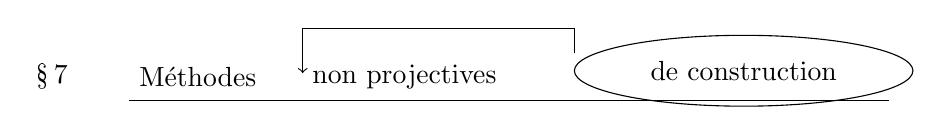
\begin{tikzpicture}[x=1cm,y=1cm]
\node[anchor=west] at (-1.3,0) {\deleted{\S\,7}};
\node[anchor=west] at (0,0) {Méthodes};
\node[anchor=west] at (2.2,0) {non projectives};
\node (construction) at (7.8,.08) {\inserted{de construction}};
\draw (construction.center) ellipse (2.15cm and .45cm);
\draw[->] (5.65,.3) -- (5.65,.62) -- (2.2,.62) -- (2.2,.05);
\draw (0,-.3) -- (9.65,-.3);
\end{tikzpicture}}

\figure{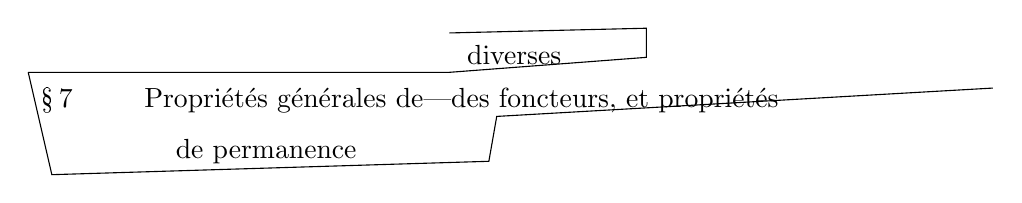
\begin{tikzpicture}[x=1cm,y=1cm]
\node[anchor=west] at (-1.3,0) {\deleted{\S\,7}};
\node[anchor=west] at (0,0) {\deleted{Propriétés générales \unsure{de|des} \unsure{foncteurs}, et propriétés}};
\node[anchor=west] at (.4,-.65) {\deleted{de permanence}};
\node[anchor=west] at (4.1,.58) {\deleted{\inserted{\unsure{diverses}}}};
\draw (-1.35,.36) -- (4.0,.36) -- (6.5,.55) -- (6.5,.92) -- (4.0,.86);
\draw (-1.35,.36) -- (-1.05,-.94) -- (4.5,-.77) -- (4.6,-.2) -- (10.9,.16);
\end{tikzpicture}}

\S\,7\quad \uline{Proreprésentabilité}: (et variantes).

\tikz[baseline=(p.base),remember picture]{\node[inner sep=1pt] (p) {\S\,\deleted{\unsure{8}}9};}\quad
\uline{Invariants différentiels} \deleted{\unsure{de|du} \unsure{div.}} \inserted{\uline{\unsure{tangts|tang.} et normaux}}

\tikz[baseline=(q10.base)]{\node[inner sep=1pt] (q10) {\S\,10};\draw (q10.center) ellipse (1.25em and .9em);}\quad
\margin{\fbox{Après \S\,12 ??}}Propriétés générales de foncteurs, \uline{propriétés de permanence}
\margin{$\left\{\begin{gathered}\text{Foncteurs \uline{excellent} sur S}\\ \text{morphismes excellent}\\ \text{??}\end{gathered}\right.$}

\tikz[baseline=(q11.base),remember picture]{\node[inner sep=1pt] (q11) {\S\,\deleted{\unsure{10|11}}11};\draw (q11.center) ellipse (1.65em and .9em);}\quad
\margin{\tikz[remember picture]{\node[draw,inner sep=2pt] (m11) {\parbox{.90\marginparwidth}{\raggedright Commun au \unsure{par.} \unsure{20|2e|éd} ? Cas Greenberg ?}};}}
Représentabilités ``élémentaires'' du type $\prod_{\deleted{X}Y/S}X/Y$.

\inserted{cf SGAD $\underline{\overline{\mathrm{VIII}}}$ 6 et $\underline{\overline{\mathrm{XI}}}$ 6.8.}

\tikz[baseline=(r.base),remember picture]{\node[draw,rounded corners,inner sep=1pt] (r) {\S\,8\deleted{\unsure{1|11}}};}
\quad Construction de Modules cohérents
\figure{\begin{tikzpicture}[remember picture,overlay]\draw[->] (r.north west) to[out=125,in=190] (p.north);\draw (q11.east) -- (m11.west);\end{tikzpicture}}

\S\,12\quad \deleted{\unsure{Représentabilité}}\inserted{Foncteurs} \unsure{repr.} par morphismes \inserted{\uline{\unsure{séparés|xprés}}} loc. pr. \unsure{f|fi}

\S\,13\quad Applications : des \unsure{th\textsuperscript{es}|th\textsuperscript{s}} \deleted{de} représentabilité relatifs. (y compris \unsure{(}pour les es foncteurs étales\ldots\unsure{,|)}

% archive sheet number: 2
